\documentclass[12pt]{article}
\usepackage{graphicx}
\usepackage[margin=1in]{geometry}
\usepackage{amsmath, amssymb} 
\usepackage{listings} 
\usepackage{xcolor} 

\lstset{
    basicstyle=\ttfamily,
    columns=fullflexible,
    frame=single,
    breaklines=true,
    postbreak=\mbox{\textcolor{red}{$\hookrightarrow$}\space},
}

\title{Mathematical Morphology Operations on Binary Images}
\author{Matteo Scardovi}
\date{\today}

\begin{document}

\maketitle

\section{Program Overview}
This program is designed to detect and recognize a Sudoku grid and its digits from an input image. It has several stages, including image preprocessing, grid detection, cell identification, and digit recognition through template matching.

\section{Elaboration Steps}

\subsection{Preprocessing}
The image is first converted to grayscale and then thresholded using adaptive Gaussian thresholding to produce a binary image. This step enhances the contrast between the grid lines and the background, facilitating the detection of edges and lines in subsequent steps.

\subsection{Detecting the Sudoku Grid}
The program employs the Canny edge detector to find edges in the preprocessed image, followed by the Hough Transform to detect lines. Lines that correspond to the Sudoku grid are then drawn on a copy of the original image for visualization.

\subsection{Finding the Coordinates of the Cells}
Horizontal and vertical lines are separated based on their orientation, and their intersections are calculated to determine the top-left corners of each cell within the grid. A method to eliminate nearby duplicate points ensures the uniqueness of cell corners.

\subsection{Recognizing Numbers}
Digit recognition is performed using template matching for each cell against preloaded templates of digits 1 through 9. The best match is determined based on a correlation coefficient, with a threshold applied to decide whether a cell contains a digit or is empty.


\section{Usage}

To use this program, you must provide at least one argument to the command line: the path to the image file containing the Sudoku puzzle. Optionally, you can also specify a custom path for templates used in number recognition.

\begin{verbatim}
    python Sudoku.py [image_path] [template_path]
\end{verbatim}

\begin{itemize}
    \item \textbf{image\_path}: Required. The path to the image file containing the Sudoku puzzle you wish to recognize.
    \item \textbf{template\_path}: Optional. The path to the directory containing templates for number recognition. If not specified, a default path of "templates/" will be used. The templates must be png files of the digits labeled 1.png through 9.png.
\end{itemize}

\section{Example}
\begin{verbatim}
    python Sudoku.py standard.png
\end{verbatim}
\begin{figure}[h!]
    \centering
    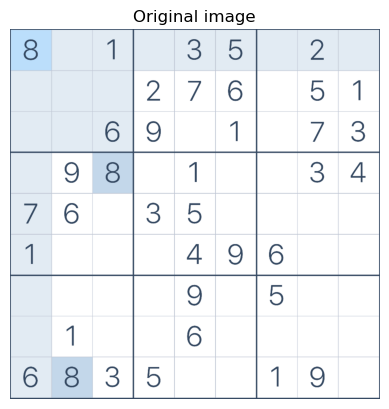
\includegraphics[width=0.5\textwidth]{original.png}
    \caption{Original sudoku image.}
\end{figure}
\begin{figure}[h!]
    \centering
    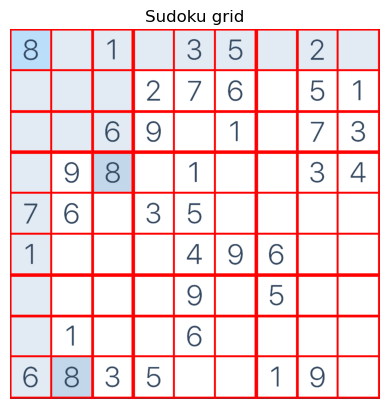
\includegraphics[width=0.5\textwidth]{grid.png}
    \caption{The grid is drawn over the original image and shown to the user.}
\end{figure}
\newpage
After number recognition, the output of the program in the CLI will be the following:

\begin{equation*}
    \begin{array}{ccccccccc}
    8 & - & 1 & - & 3 & 5 & - & 2 & - \\
    - & - & - & 2 & 7 & 6 & - & 5 & 1 \\
    - & - & 6 & 9 & - & 1 & - & 7 & 3 \\
    - & 9 & 8 & - & 1 & - & - & 3 & 4 \\
    7 & 6 & - & 3 & 5 & - & - & - & - \\
    1 & - & - & - & 4 & 9 & 6 & - & - \\
    - & - & - & - & 9 & - & 5 & - & - \\
    - & 1 & - & - & 6 & - & - & - & - \\
    6 & 8 & 3 & 5 & - & - & 1 & 9 & - \\
    \end{array}
\end{equation*}


\end{document}
